% vim: spelllang=es

\chapter{Entendiendo Tremor}\label{ch:tremor}

\section{Sistemas de Procesado de Eventos}

Tremor es un \emph{Sistema de Procesado de Eventos}, que consiste en ``el
monitorizado y análisis (procesado) de flujos de información (datos) sobre cosas
que pasan (eventos)''~\cite{luckham2011event}. Tremor fue creado como una
alternativa de alto rendimiento a herramientas como \textcite{logstash} o
\textcite{telegraf}, pero ha evolucionado para soportar casos de uso más
complejos. Al contrario que esas piezas de software, Tremor también tiene
soporte para \emph{agregación} y \emph{rollups}, e incluye un lenguaje \emph{ad
hoc} para \emph{Extract, Transform, and Load (ETL)} y consultas.

Para más información sobre Tremor se puede consultar \textcite{tremorintro}, que
contiene una explicación de sus conceptos más básicos y sus posibles usos --- o
cuándo \emph{no} usarlo, en \textcite{tremorconstraints}.
\textcite{tremorrecipes} lista un total de 32 ejemplos de cómo configurar y
emplear el software.

La figura~\ref{fig:tremor_example} ilustra uno de los casos de uso más básicos
de Tremor:

\begin{enumerate}
    \item Recibir \emph{logs} de aplicaciones con diferentes protocolos o
        formatos en una empresa.
    \item Filtrar los casos redundantes, añadir campos y eliminar algunos
        innecesarios, y transformar a un mismo formato.
    \item Enviar todos los logs estructurados a una base de datos para
        analizarlos posteriormente.
\end{enumerate}

\begin{figure}
    \centering
    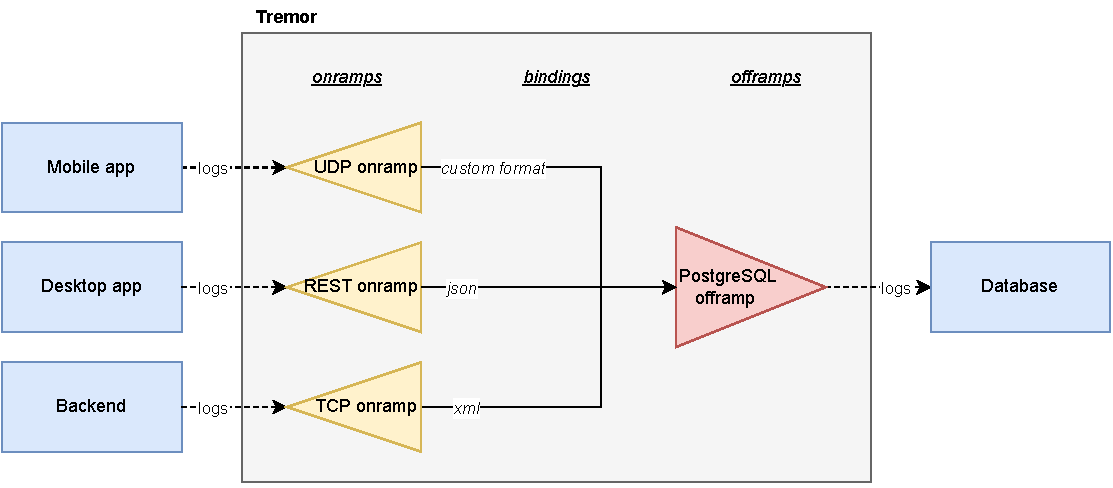
\includegraphics[width=\textwidth]{./Imagenes/example.pdf}
    \caption{Ejemplo de uso de Tremor}%
    \label{fig:tremor_example}
\end{figure}

\begin{figure}
    \centering
    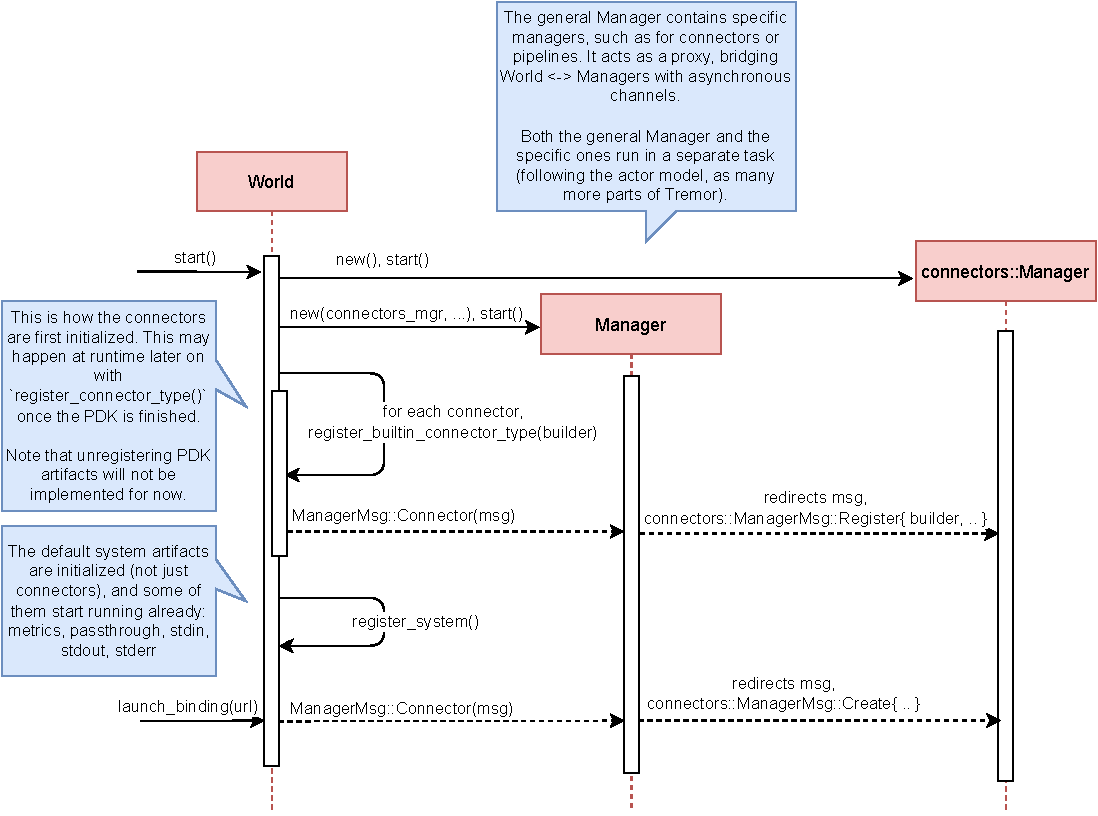
\includegraphics[width=\textwidth]{./Imagenes/registering.pdf}
    \caption{Ejemplo de uso de Tremor}%
    \label{fig:tremor_registering}
\end{figure}

\begin{figure}
    \centering
    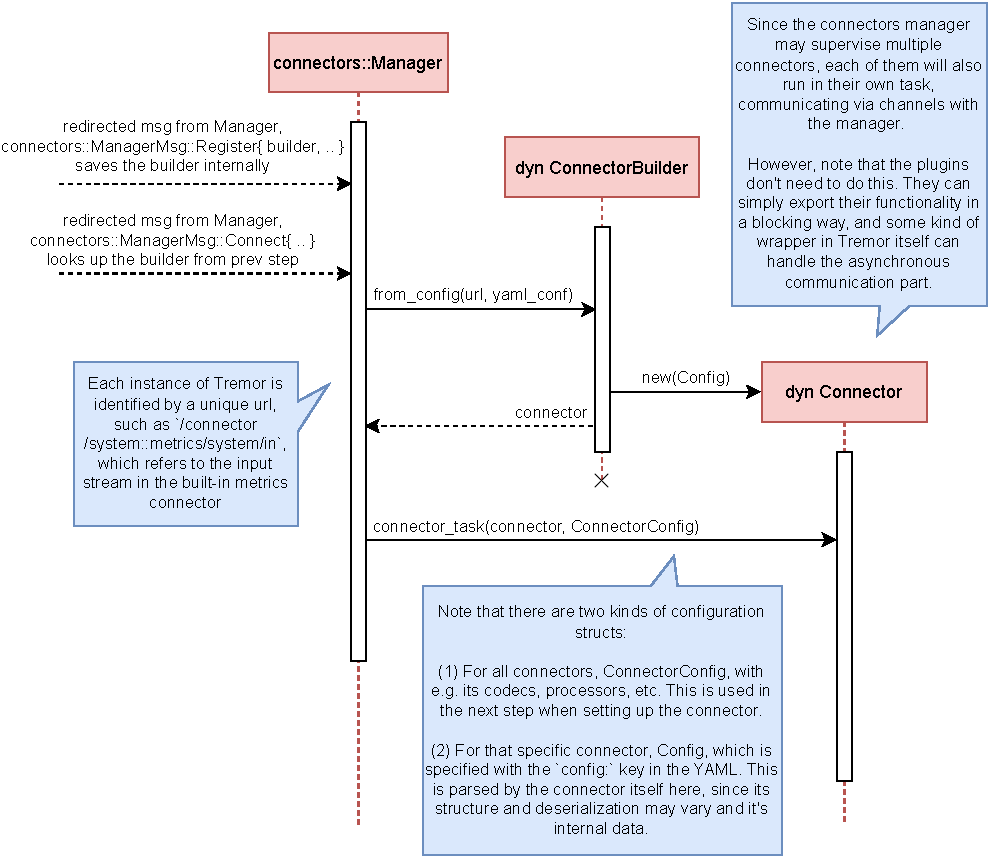
\includegraphics[width=\textwidth]{./Imagenes/initializing.pdf}
    \caption{Ejemplo de uso de Tremor}%
    \label{fig:tremor_initializing}
\end{figure}

\begin{figure}
    \centering
    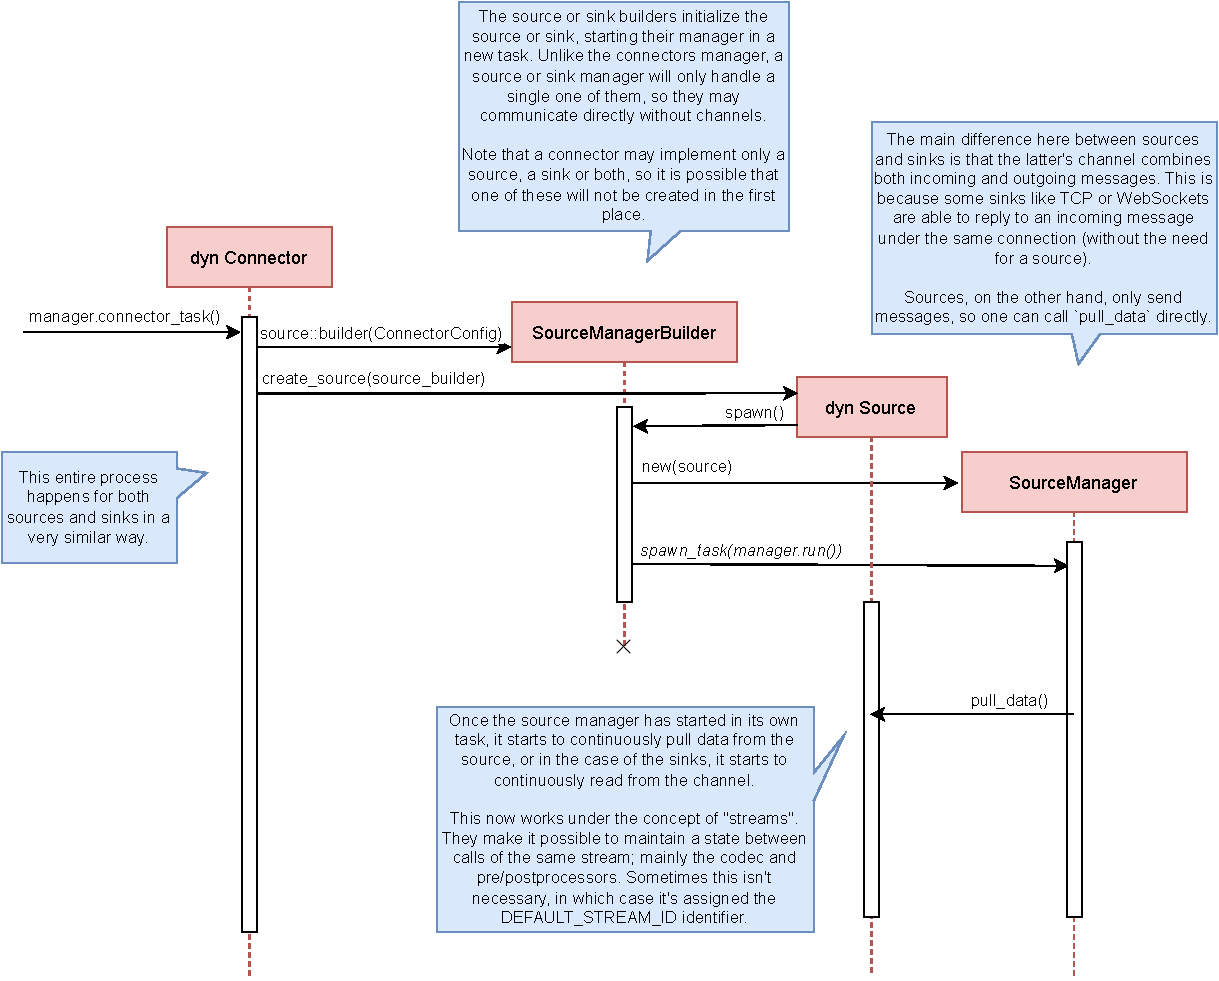
\includegraphics[width=\textwidth]{./Imagenes/setting-up.pdf}
    \caption{Ejemplo de uso de Tremor}%
    \label{fig:tremor_setting_up}
\end{figure}
